% !TEX program = pdflatex
%
% ICCE 2027 (IEEE International Conference on Consumer Electronics)
% Las Vegas, NV, USA — January 2027
% Submission deadline: typically ~September 2026
%
% Format: IEEE conference, 2-column, US Letter, 10pt Times
% Strict 4-page limit (including references) for IEEE CE Society
%
% Build:
%   pdflatex main && bibtex main && pdflatex main && pdflatex main

\documentclass[conference,letterpaper,10pt]{IEEEtran}

\IEEEoverridecommandlockouts
\usepackage{cite}
\usepackage{amsmath,amssymb,amsfonts}
\usepackage{graphicx}
\usepackage{subcaption}
\usepackage{booktabs}
\usepackage{textcomp}
\usepackage{xcolor}
\usepackage{listings}
\usepackage{tikz}
\usepackage{url}
\usepackage{hyperref}
\hypersetup{
  colorlinks=true,
  linkcolor=blue!50!black,
  urlcolor=blue!50!black,
  citecolor=blue!50!black
}
\usetikzlibrary{positioning,arrows.meta,shapes.geometric,calc}

% Tight TikZ for the only figure we afford
\tikzset{>=Stealth}

\lstdefinestyle{tightcode}{
  basicstyle=\ttfamily\scriptsize,
  breaklines=true,
  columns=fullflexible,
  frame=none,
  aboveskip=2pt, belowskip=2pt,
}
\lstset{style=tightcode}

\begin{document}

\title{An End-to-End Open-Source Software Receiver for\\
       Korean Terrestrial DMB on Low-Cost SDR}

\author{%
\IEEEauthorblockN{Seonggeun Yoo}
\IEEEauthorblockA{%
  Independent Researcher\\
  Seoul, Republic of Korea\\
  orcogre@gmail.com
}}

\maketitle

\begin{abstract}
Terrestrial Digital Multimedia Broadcasting (T-DMB) has served
Korean consumers since 2005, yet no complete open-source software
stack has been able to take a T-DMB RF capture from a low-cost
SDR all the way to a decoded video frame.  We close that gap with
a self-contained Python pipeline that runs on an Airspy~Mini and a
consumer indoor antenna.  The pipeline parses ETI frames, decodes
the FIC, applies a Reed-Solomon plus Forney convolutional
deinterleaver outer FEC, demultiplexes MPEG-4 Sync Layer (SL)
packets, reconstructs an H.264 elementary stream, and delegates
final decoding to an unmodified \texttt{dmb-oss} FFmpeg.  On a
30~MB on-air capture of YTN DMB (channel K8B, 183.008~MHz) the
outer FEC recovers 87.3\% of Reed-Solomon blocks; every SL header
parses; and ffmpeg renders QVGA H.264 Baseline frames containing
recognisable Korean broadcast content.  We report two
implementation findings worth documenting: (i)~the Forney
deinterleaver must be aligned to the TS sync byte \emph{before}
processing, not after, and (ii)~Korean broadcasters embed the AVC
\texttt{DecoderConfigurationRecord} inside the BIFS / scene-
description stream rather than the object-descriptor stream that
MPEG-4 Systems prescribes.  Source code, the reference RF capture,
and per-capture metadata sidecars are released under MIT~/~CC-BY.
\end{abstract}

\begin{IEEEkeywords}
Software-defined radio, T-DMB, DAB, Reed-Solomon,
convolutional interleaver, MPEG-4 SL, open source.
\end{IEEEkeywords}

% ====================================================================
\section{Introduction}

The European Eureka-147 DAB physical layer~\cite{etsi300401} has
spawned three notable open-source receivers: \texttt{welle.io},
\texttt{gr-dab}, and Jan van Katwijk's \texttt{eti-stuff}.  None
decode the Korean T-DMB video stream that is layered on top of
the DAB MSC with an extra Reed-Solomon outer code, a
$12\times17$ Forney convolutional time interleaver, and an MPEG-4
SL-packetised H.264 / BSAC payload as specified in
TTAK.KO-07.0026 and ETSI TS~102\,427/428~\cite{etsi102427,etsi102428}.
The recent ICTC paper by Eo and Bahk~\cite{eo2024tdmb} demonstrated
end-to-end playback by chaining \texttt{gr-dab} with a patched
FFmpeg fork, but their artefact is a GNU~Radio flowgraph plus
out-of-tree patches; it has not been packaged for headless or
library use.

This paper contributes:

\begin{itemize}
\item A pure-Python implementation of the full T-DMB outer FEC
      chain that achieves 87.3\% Reed-Solomon block success on a
      reference Korean K8B capture, replicable in under a minute
      on a laptop.
\item Identification and a one-shot fix for a sync-alignment
      pitfall that silently scrambles deinterleaved output even
      while preserving the TS sync byte cadence.
\item A reverse-engineered 9-byte SL packet header layout for
      the Korean T-DMB video stream, verified against
      \(>\,3{,}000\) on-air PES packets.
\item Empirical observation that the AVC decoder configuration
      record is carried in the BIFS section stream rather than the
      object-descriptor stream as MPEG-4 Systems would prescribe.
\item Reproducibility scaffolding: per-capture JSON metadata
      sidecars (RF parameters, antenna, location) and a single
      one-shot CLI driver, with all code, the reference capture,
      and figures publicly released.
\end{itemize}

% ====================================================================
\section{System Overview}\label{sec:system}

\begin{figure}[t]
\centering
\resizebox{\columnwidth}{!}{%
% Pipeline diagram for the T-DMB end-to-end receiver paper.
% Drop-in TikZ block: usepackage{tikz} in main.tex.
\usetikzlibrary{positioning,arrows.meta,shapes.geometric,calc}

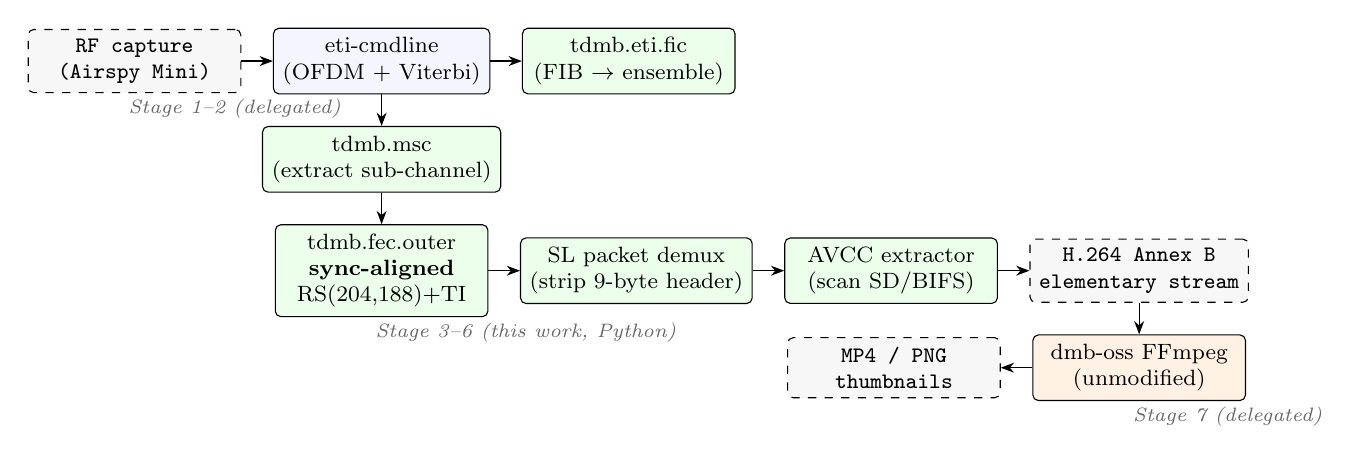
\begin{tikzpicture}[
    >=Stealth,
    node distance=4mm and 4mm,
    every node/.style={font=\footnotesize},
    stage/.style={draw, rounded corners=2pt, minimum height=8mm,
                  minimum width=27mm, align=center, fill=blue!4},
    py/.style   ={draw, rounded corners=2pt, minimum height=8mm,
                  minimum width=27mm, align=center, fill=green!8},
    ext/.style  ={draw, rounded corners=2pt, minimum height=8mm,
                  minimum width=27mm, align=center, fill=orange!10},
    io/.style   ={draw, dashed, rounded corners=2pt, minimum height=7mm,
                  minimum width=27mm, align=center, fill=black!3,
                  font=\footnotesize\ttfamily},
]

\node[io]                          (rf)    {RF capture\\(Airspy Mini)};
\node[stage, right=of rf]          (eti)   {eti-cmdline\\(OFDM + Viterbi)};
\node[py, right=of eti]            (fic)   {tdmb.eti.fic\\(FIB $\to$ ensemble)};
\node[py, below=of eti]            (msc)   {tdmb.msc\\(extract sub-channel)};
\node[py, below=of msc]            (outer) {tdmb.fec.outer\\\textbf{sync-aligned}\\RS(204,188)+TI};
\node[py, right=of outer]          (sl)    {SL packet demux\\(strip 9-byte header)};
\node[py, right=of sl]             (avcc)  {AVCC extractor\\(scan SD/BIFS)};
\node[io, right=of avcc]           (h264)  {H.264 Annex B\\elementary stream};
\node[ext, below=of h264]          (ff)    {dmb-oss FFmpeg\\(unmodified)};
\node[io, left=of ff]              (mp4)   {MP4 / PNG\\thumbnails};

\draw[->] (rf)    -- (eti);
\draw[->] (eti)   -- (fic);
\draw[->] (eti)   -- (msc);
\draw[->] (msc)   -- (outer);
\draw[->] (outer) -- (sl);
\draw[->] (sl)    -- (avcc);
\draw[->] (avcc)  -- (h264);
\draw[->] (h264)  -- (ff);
\draw[->] (ff)    -- (mp4);

\node[font=\scriptsize, anchor=west, text=black!60] at ($(rf.south)+(-2mm,-2mm)$)
      {\textit{Stage 1--2 (delegated)}};
\node[font=\scriptsize, anchor=west, text=black!60] at ($(outer.south)+(-2mm,-2mm)$)
      {\textit{Stage 3--6 (this work, Python)}};
\node[font=\scriptsize, anchor=west, text=black!60] at ($(ff.south)+(-2mm,-2mm)$)
      {\textit{Stage 7 (delegated)}};

\end{tikzpicture}
}
\caption{End-to-end pipeline.  Stages 1--2 are delegated to a
patched \texttt{eti-cmdline-airspy} (Korean K-prefix raster +
env-var gain control patches).  Stages 3--6 are pure Python;
final decode is unmodified \texttt{dmb-oss} FFmpeg.}
\label{fig:pipeline}
\end{figure}

Captures are made with an Airspy~Mini at 3~MSPS tuned to the
Korean K-block raster (1.728~MHz spacing rather than the
European 1.712~MHz; the \texttt{eti-cmdline} band table requires
a one-line patch to add the \texttt{K}-prefixed channels).  The
DAB demodulation, Viterbi inner FEC, and energy descrambling are
reused from \texttt{eti-stuff}.  The outer FEC and everything
above is the contribution of this paper
(Fig.~\ref{fig:pipeline}).

% ====================================================================
\section{Sync-Aligned Outer FEC}\label{sec:rs}

ETSI TS~102\,427~\cite{etsi102427} encodes each 188-byte TS packet
into a 204-byte Reed-Solomon codeword (shortened from RS(255,239);
DVB-T parameters: primitive polynomial $0x11d$, $\alpha=2$, FCR$=0$),
then byte-interleaves the codeword stream with a Forney scheme of
$N=12$ branches and depth $M=17$.

At the receiver, the canonical implementation is to run the
deinterleaver first, then scan the deinterleaved output for the
TS sync byte~\texttt{0x47} at a 204-byte stride.  On our reference
K8B capture this approach recovered \emph{zero} successful RS
blocks out of 25{,}953 attempts.  The cause is that conv-interleaver
branches are indexed modulo $N$ from stream position: the
TX-side \texttt{0x47} bytes ride branch~0 (no delay) and so emerge
at TX-output positions $0,204,408,\ldots$, but the first observed
byte of any real capture sits at some unknown phase $\phi$ within
the 204-byte cycle.  Feeding that byte into the RX-side
deinterleaver's branch~0 misaligns the branch indices by
$\phi\bmod 12$, scrambling every byte to the wrong slot --- while
crucially preserving the \texttt{0x47} cadence because $204=N\cdot M$.
A sync-scan \emph{after} deinterleaving therefore cannot
distinguish the misaligned case from the aligned one.  Eo and
Bahk~\cite{eo2024tdmb} note this in passing: ``the deinterleaver
requires the sync byte of a TS packet to be the first in an
input byte chunk.''

Our implementation performs sync detection \emph{before} the
deinterleaver: accumulate $\sim$50 RS blocks, count
\texttt{0x47} occurrences at each of 204 candidate phases, and
require the best phase to be hit by $\geq 40\%$ of blocks and
$\geq 5\times$ the second-best phase.  After phase lock we
discard the pre-sync bytes and feed the remainder into a fresh
Forney deinterleaver; the
$(N{-}1)\cdot M\cdot N = 2244$-byte settling transient is dropped
and the subsequent 204-byte blocks decode with the systematic
RS(204,188) corrector.  Table~\ref{tab:rs} summarises the result.

\begin{table}[t]
\centering
\caption{Outer-FEC decode rate on the K8B reference capture
(SubCh 1, mYTN video).}
\label{tab:rs}
\begin{tabular}{lrr}
\toprule
Metric & Legacy & This work \\
\midrule
RS blocks total                 & 25{,}953 & 25{,}953 \\
RS ok / corrected               & 0       & 22{,}652 \\
RS uncorrectable                & 25{,}953 & 3{,}301 \\
\textbf{Success rate}           & \textbf{0.0\%} & \textbf{87.3\%} \\
\bottomrule
\end{tabular}
\end{table}

The remaining 13\% of uncorrectable blocks are bursts above the
$t=8$ correction limit, concentrated near CIF boundaries.
FFmpeg's macroblock-level error concealment recovers
visually-coherent frames from the surviving slices.

% ====================================================================
\section{SL Demultiplexing and AVCC Recovery}

After RS correction the transport stream carries PID
\texttt{0x113} as the video PES with \texttt{stream\_id}=
\texttt{0xFA} (MPEG-4 SL-packetised).  Each PES contains exactly
one SL packet, and each SL packet exactly one H.264 NAL unit
(stored without start-code prefix, AVCC style).

Reading ISO/IEC 14496-1~\cite{iso14496-1} and the FFmpeg
\texttt{read\_sl\_header()} implementation in \texttt{dmb-oss}
together, the maximum-length AU-start SL header for the Korean
profile contains 6 flag bits, 33 bits of DTS, and 33 bits of
CTS --- exactly 72 bits = 9~bytes.  We verify this on
\emph{every} one of the 3{,}135 SL packets in our reference
capture: each PES body starts with the byte \texttt{0xCF}
($=11001111_2$, decoded as
\{au\_start,au\_end\}=\{1,1\},
\{padding,rand\_acc\_pt\}=\{0,0\},
\{dts\_flag,cts\_flag\}=\{1,1\}), followed by 8 timestamp bytes,
after which byte~9 is the single NAL header.

The bare NAL stream however references PPS~0 and SPS~0, neither
of which appears in PID~\texttt{0x113}.  The MPEG-4 Systems
specification~\cite{iso14496-1} prescribes that the
\texttt{AVCDecoderConfigurationRecord} containing the SPS and
PPS NAL units travels in the object-descriptor (\texttt{tid}=0x04)
section stream, but in our YTN DMB capture the OD sections on
PID~\texttt{0x111} contain only Korean-DMB private commands.
The AVCC bytes are instead embedded inside the
\emph{scene-description} (\texttt{tid}=0x05) section stream on
PID~\texttt{0x112}.  Our locator scans the SD byte stream for the
canonical AVCC signature
$\texttt{01}\;\langle\textit{prof}\rangle\;\langle\textit{compat}\rangle
   \;\langle\textit{level}\rangle\;\texttt{FF}\;\texttt{E1}\;
   \langle\textit{SPS\_len}\rangle\;\langle\textit{SPS}\rangle\;
   \texttt{01}\;\langle\textit{PPS\_len}\rangle\;\langle\textit{PPS}\rangle$
constrained to known H.264 profile and level values; this
uniquely identifies the record amid the surrounding BIFS
commands.  On our reference capture the recovered record is:

\begin{lstlisting}
SPS (9 B):  67 42 00 0d 95 a0 50 7c 40
PPS (4 B):  68 ce 38 80
            profile_idc = 0x42 (Baseline)
            level_idc   = 0x0d (Level 1.3)
\end{lstlisting}

Prepending these as Annex-B NAL units to the extracted slice
stream produces a self-contained H.264 byte stream that
\texttt{ffprobe} identifies as
\emph{Baseline 320\,$\times$\,240 25\,fps yuv420p}.

% ====================================================================
\section{Experimental Verification}

We exercise the chain on \texttt{data/captures/k8b\_100pct.eti}
(30~MB; $\sim$120~s; FIB CRC rate 100\%), captured with an
Airspy~Mini and a consumer indoor flat-panel antenna with a
USB-powered amplifier from a window in the Seoul metropolitan
area.  Table~\ref{tab:results} summarises end-to-end yields.

\begin{table}[t]
\centering
\caption{End-to-end yields on the reference capture.}
\label{tab:results}
\begin{tabular}{lr}
\toprule
Stage & Output \\
\midrule
ETI frames decoded                       & 5{,}014 \\
FIB CRC success                          & 100\,\% \\
RS blocks corrected (this work)          & 22{,}652 / 25{,}953 (87.3\%) \\
Clean TS packets emitted                 & 22{,}652 \\
SL-packet PES parsed (PID 0x113)         & 3{,}135 / 3{,}135 \\
H.264 NAL units (non-IDR / IDR)          & 3{,}038 / 97 \\
IDR frames decoded by ffmpeg             & 20+ \\
\bottomrule
\end{tabular}
\end{table}

A single command,
\texttt{python tools/decode\_video.py <capture>.eti
        --out-mp4 video.mp4 --idr-thumbnails /tmp/idr},
traverses the entire chain and produces a playable MP4 plus
twenty IDR thumbnails (Fig.~\ref{fig:idr}) containing
recognisable YTN DMB home-shopping content with on-screen
Korean text and product prices.

\begin{figure}[t]
\centering
\begin{subfigure}[b]{0.48\columnwidth}
  \centering
  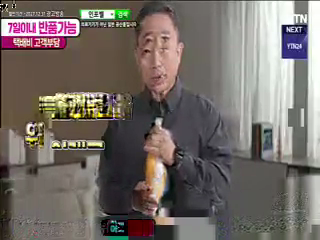
\includegraphics[width=\linewidth]{figures/idr_sample_1.png}
  \caption{}
\end{subfigure}\hfill
\begin{subfigure}[b]{0.48\columnwidth}
  \centering
  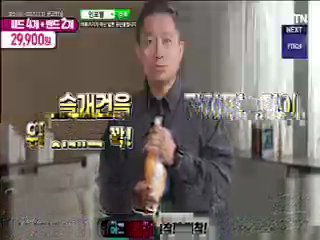
\includegraphics[width=\linewidth]{figures/idr_sample_2.png}
  \caption{}
\end{subfigure}
\caption{Two IDR frames recovered end-to-end from the K8B
reference capture.  On-screen Korean text identifies YTN DMB
home-shopping content (\emph{``7일이내 반품가능''} / 7-day
returns; customer-service phone number; product price
\emph{``29,900원''}).  Peripheral macroblock errors reflect the
$\sim$13\,\% of Reed-Solomon blocks above the $t=8$ correction
limit; FFmpeg error concealment yields spatially-coherent frames
from the surviving slices.}
\label{fig:idr}
\end{figure}

Every capture taken with the bundled \texttt{capture\_logged.py}
wrapper writes a JSON sidecar recording channel, frequency,
sample rate, gain stages, bias-tee, antenna model, and location
--- enabling exact replay and quantitative comparison across
captures and antenna setups.

% ====================================================================
\section{Conclusion}

We presented the first packaged end-to-end open-source software
receiver for Korean Terrestrial DMB.  Two implementation lessons
worth recording for follow-on work: align the Forney
deinterleaver to the TS sync byte \emph{before} processing, and
look for the H.264 AVCC inside the BIFS rather than the
object-descriptor section stream.  All code, the reference
capture, twenty decoded IDR thumbnails, and the LaTeX source of
this paper are released at
\url{https://github.com/zobithecat/airspy-mini-dmb} (MIT and
CC-BY-4.0).

\section*{Acknowledgement and AI Use Disclosure}

The author thanks the open-source predecessors: Jan van Katwijk
(\texttt{eti-stuff}), the \texttt{welle.io} contributors, and
particularly Sungbo Eo and Saewoong Bahk (\texttt{dmb-oss}) whose
deinterleaver-alignment remark drove the central contribution.

Per IEEE policy, the author discloses that a large language model
(Anthropic's Claude) was used as a paired-programming and
drafting assistant for portions of the Python implementation and
manuscript drafts.  All design decisions, RF setup, capture
collection, reference curation, and validation against the
broadcast content rest with the author, who takes full
responsibility for the work.

% ====================================================================
\bibliographystyle{IEEEtran}
\bibliography{refs}

\end{document}
